%Admittedly, structure learning is an overloaded term, so in this chapter, we aim to define it and provide example problems. We will also identify and focus on its Bayesian variant.
In this chapter we define the Bayesian structure learning problem and cover relevant technical background material.

\section{What is structure learning?}
Learning structure is a broad problem; we define it as an unsupervised learning problem wherein a user has data
and a priori assumes some unobserved, or \emph{latent}, organization of the data. Example organizations of the data might include a flat clustering, i.e. the data can be partitioned into some $\k$ distinct groups. A logical extension of a flat clustering organization is a mixed-membership model, where data can be organized into $\k$ groups but each datum may belong to many groups simultaneously. 
In this thesis, we are particularly interested in hierarchical clustering, where data are organized into a tree structure, with data closer on the tree being logically or semantically similar and in
linear dynamical systems, wherein time-series data
evolve according to a linear transition function.

A structure learning problem first begins with data, and an assumption of a structure class. It then recovers a plausible structure and returns it to the user. Formally, we assume a structure class $\structures$ and return a candidate structure $\structure \in \structures$.
%In a structure learning problem, corresponding algorithms exist which have various properties and trade-offs. 
Perhaps the most famous is the $\k$-means problem, which assumes $\k$ discrete clusters to which the data belong. The corresponding algorithm recovers a $\k$-partition of the data.  Analogously in mixed-membership modeling, latent Dirichlet allocation (LDA) recovers a topic model structure for text data.

We formalize structure learning probabilistically. We will later cover the Bayesian variant, but in vanilla structure learning,
there exists some latent structure $\structure$
and a likelihood function $\p(\dataset \given \structure)$.
Recovering a structure amounts to
maximizing likelihood, i.e.
\begin{align*}
    \structure^* = \argmax_{\structure} \p(\dataset \given \structure)
\end{align*}
We now outline two structure learning problems
which are particularly relevant to this thesis. We first introduce the structure classes and present a potential likelihood function. We then discuss the relevant
algorithms that actually perform
the maximum likelihood optimization.

\subsection{Linear dynamical system}
In a linear dynamical system (LDS), 
each observed data point is a sequence, 
$\x = \sequence$, and our dataset
is a collection of $\numdata$ such sequences, $\data = \sequencen$.
The underlying structure class is
a linear-Gaussian transition function $p(\state_{\t + 1} \given \state_t, \dynmat, \dyncovar) = \N(\dynmat \state_\t, \dyncovar)$ with learnable parameters $\dynmat, \dyncovar$.
Although the underlying structure in this situation
is not discrete, as in the case
of flat or hierarchical clusterings, it is still
an assumption about the organization of data. Intuitively,
an LDS structure implies that data that temporally
close to each other are a simple transition away from each other.
Structure learning in an LDS amounts
to solving the maximum
likelihood problem
\begin{align*}
    \dynmat^*, \dyncovar^* = \argmax_{\dynmat, \dyncovar} \prod_{n = 1}^N \prod_{\t = 1}^{\T - 1} \p(\state^{(\n)}_{\t + 1} \given \state^{(\n)}_\t, \dynmat, \dyncovar)
\end{align*}
and lends itself to a closed-form solution, namely
linear regression. This formulation can also be visualized 
as a graphical model, shown in \autoref{fig:graphical-model-lds}.

\begin{figure}[htp!]
    \centering
    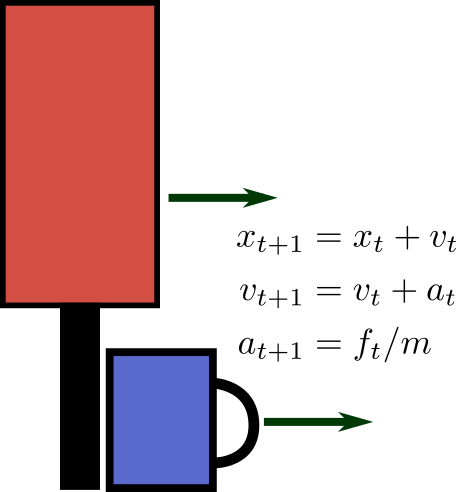
\includegraphics{tikz/lds}
    \caption{The graphical model for a linear dynamic system}
    \label{fig:graphical-model-lds}
\end{figure}

\subsection{Hierarchical clustering}
Hierarchical clustering is a structure learning problem
where the structure class is trees. Specifically,
given a dataset $\dataset$,
we are interested in rooted trees with $\numdata$ leaves
with each leaf corresponding to a data point.
Such a tree tree encodes relationships between data: 
if data points $a$ and $b$ are close in data space, we'd hope
the leaves corresponding to $a$ and $b$ appear closer
together in a tree that captures the data's structure.

Algorithms for hierarchical clustering can be broadly
divided into two categories: divisive and agglomerative.
Divisive, or top-down, clustering algorithms recover a tree by recursively
partitioning data until just leaves remain. Examples
include spectral clustering \citep{} and recursive $\k$-means.
Agglomerative, or bottom-up, clustering algorithms
initialize clusters as leaves, and recursively
merge clusters until a full binary tree is formed.
Pairs of clusters to merge are chosen according to
a heuristic, also called a linkage-criterion,
an example of which is single-linkage,
where clusters are merged according to the minimum
distance between data points in each cluster.

Hierarchical clustering can also be formalized as an optimization problem
by minimizing carefully constructed cost
function,
$C(\structure, \dataset)$,
as shown in \citet{Dasgupta2016}.
Treating this cost as a negative
energy in a Gibbs distribution,
we can also frame hierarchical clustering
as a probabilistic model
$\p(\dataset \given \tree) = \exp{-C(\tau, \dataset)/T}$ for some temperature $T$.
Recovering a hierarchical clustering of the
data is therefore a maximum likelihood problem:

\begin{align*}
    \tree^* = \argmax_{\tree} \exp{-C(\tau, \dataset)/T}
\end{align*}

\citet{Dasgupta2016} uses a greedy algorithm
to optimize this likelihood.
The graphical model for hierarchical clustering is pictured in \autoref{fig:graphical-model-hc}.

\begin{figure}[htp!]
    \centering
    \includegraphics{tikz/hc}
    \caption{Graphical model for hierarchical clustering}
    \label{fig:graphical-model-hc}
\end{figure}

\section{Bayesian structure learning}

Structure learning is an useful generalization
of several popular problems. However, it has some
drawbacks in its presented formulation.
Consider a dataset that has ambiguity in its
latent structure. For example, in \autoref{fig:ambiguous-structure}, we picture two examples of ambiguous latent structure. In a hierarchical clustering problem, if data are positioned in particular ways, we could organize the data
in several plausible ways. In one example, tare
three equally valid hierarchical clusterings (using binary trees), and in the second example, there are two
plausible clusterings. Structure learning as presented
cannot disambiguate between equally valid clusterings or indicate to a user that there exist alternative candidates.

\begin{figure*}[htp!]
    \centering
    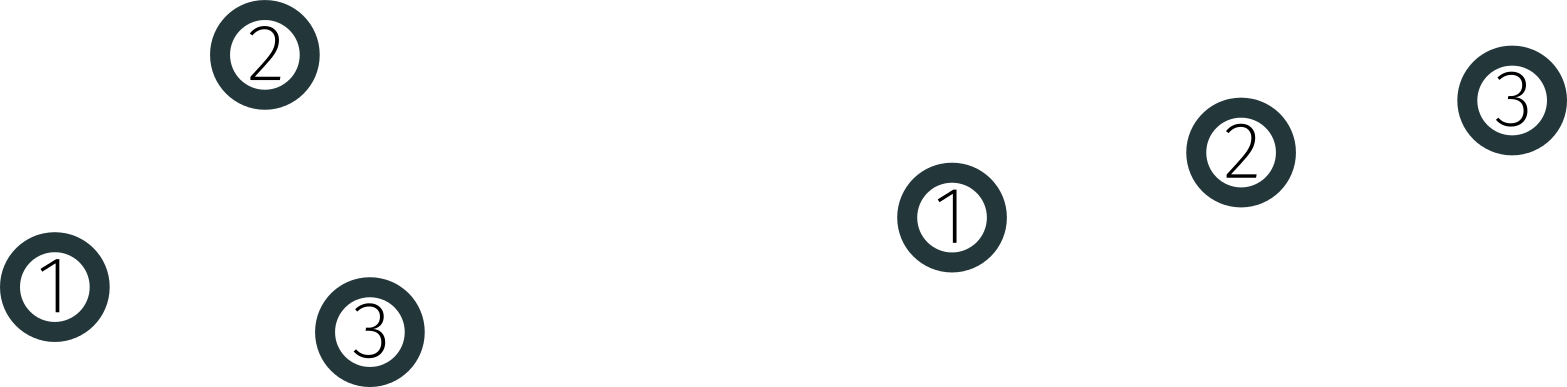
\includegraphics[width=0.8\textwidth]{img/structure/3-cluster-both}
    \caption{Examples of ambiguous hierarchical structure in data. The left set of points could plausibly be hierarchically clustered in three different ways, where any two points could be clustered before the other. The right set of points has two plausible hierarchical clusterings, where 1 and 2 could be clustered first, or 2 and 3 could be clustered first.}
    \label{fig:ambiguous-structure}
\end{figure*}

Bayesian structure learning puts a prior on the structure class $\p(\structure)$, and rather than
returning a candidate structure $\structure^*$,
it returns a posterior distribution over candidate
structures $\p(\structure \given \dataset)$. It generalizes 
vanilla structure learning, as $\p(\structure \given \dataset)$ could,
in principle,
be a delta distribution for a single candidate structure.
In practice, however, the Bayesian structure learning
formulation enables algorithms that capture
uncertainty and ambiguity in how data is organized.
In \autoref{fig:ambiguous-structure-probability},
we picture the same ambiguous hierarchical clusterings
along with the intuitively correct distribution over possible clusterings. 

\begin{figure*}[htp!]
    \centering
    \begin{subfigure}{\textwidth}
        \centering
        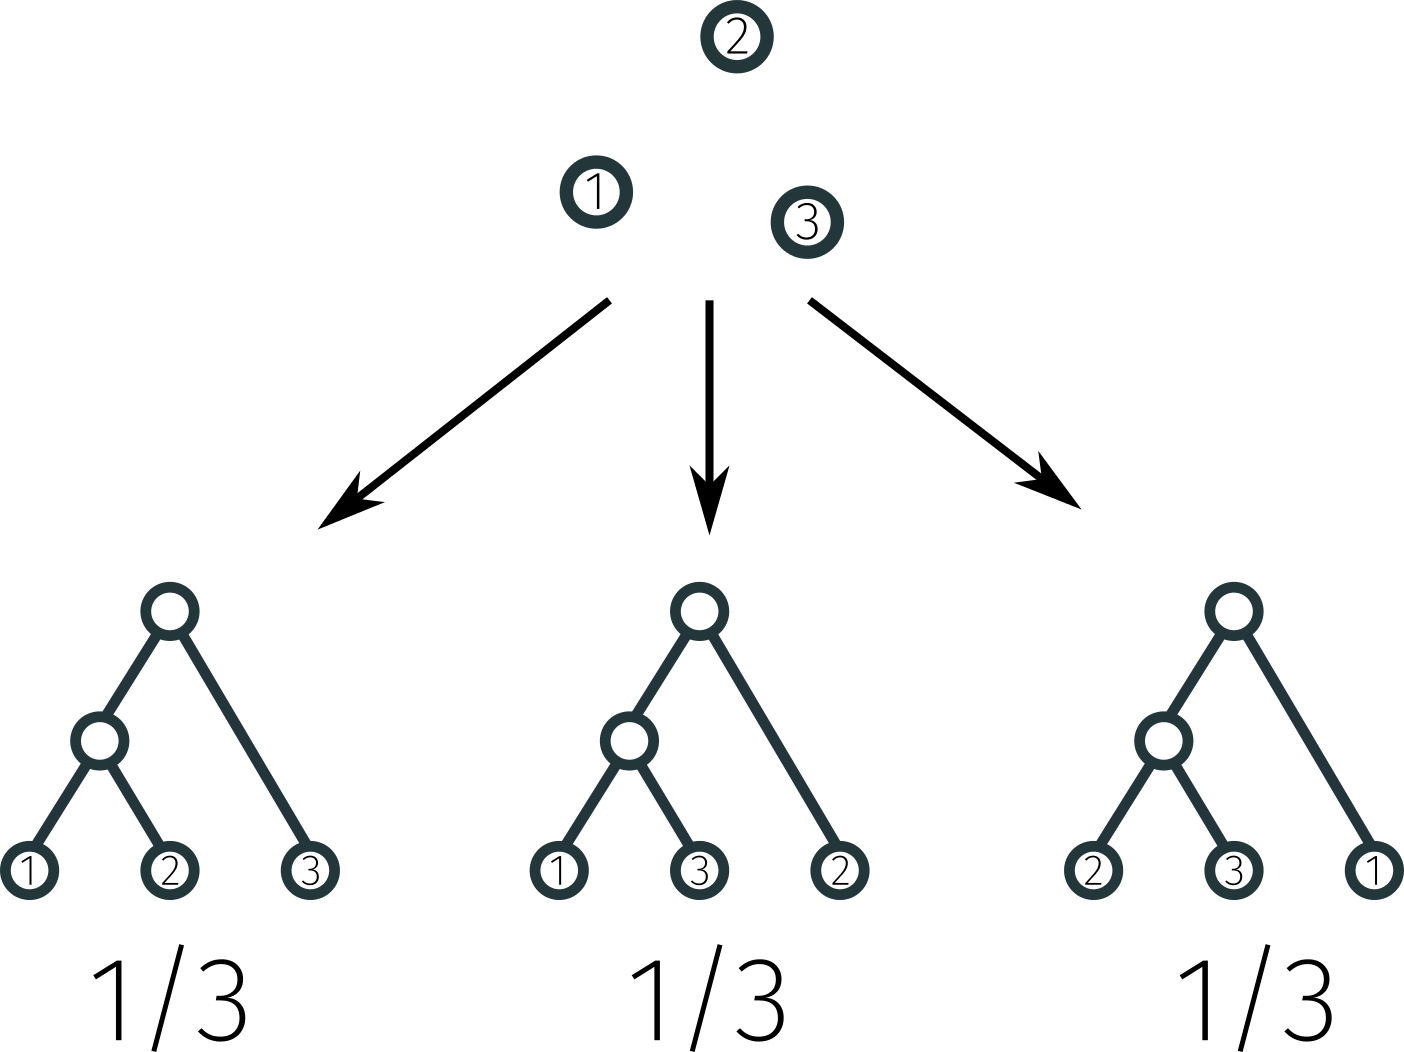
\includegraphics[width=0.7\textwidth]{img/structure/3-cluster-distribution}
        \caption{}
    \end{subfigure}
    \begin{subfigure}{\textwidth}
        \centering
        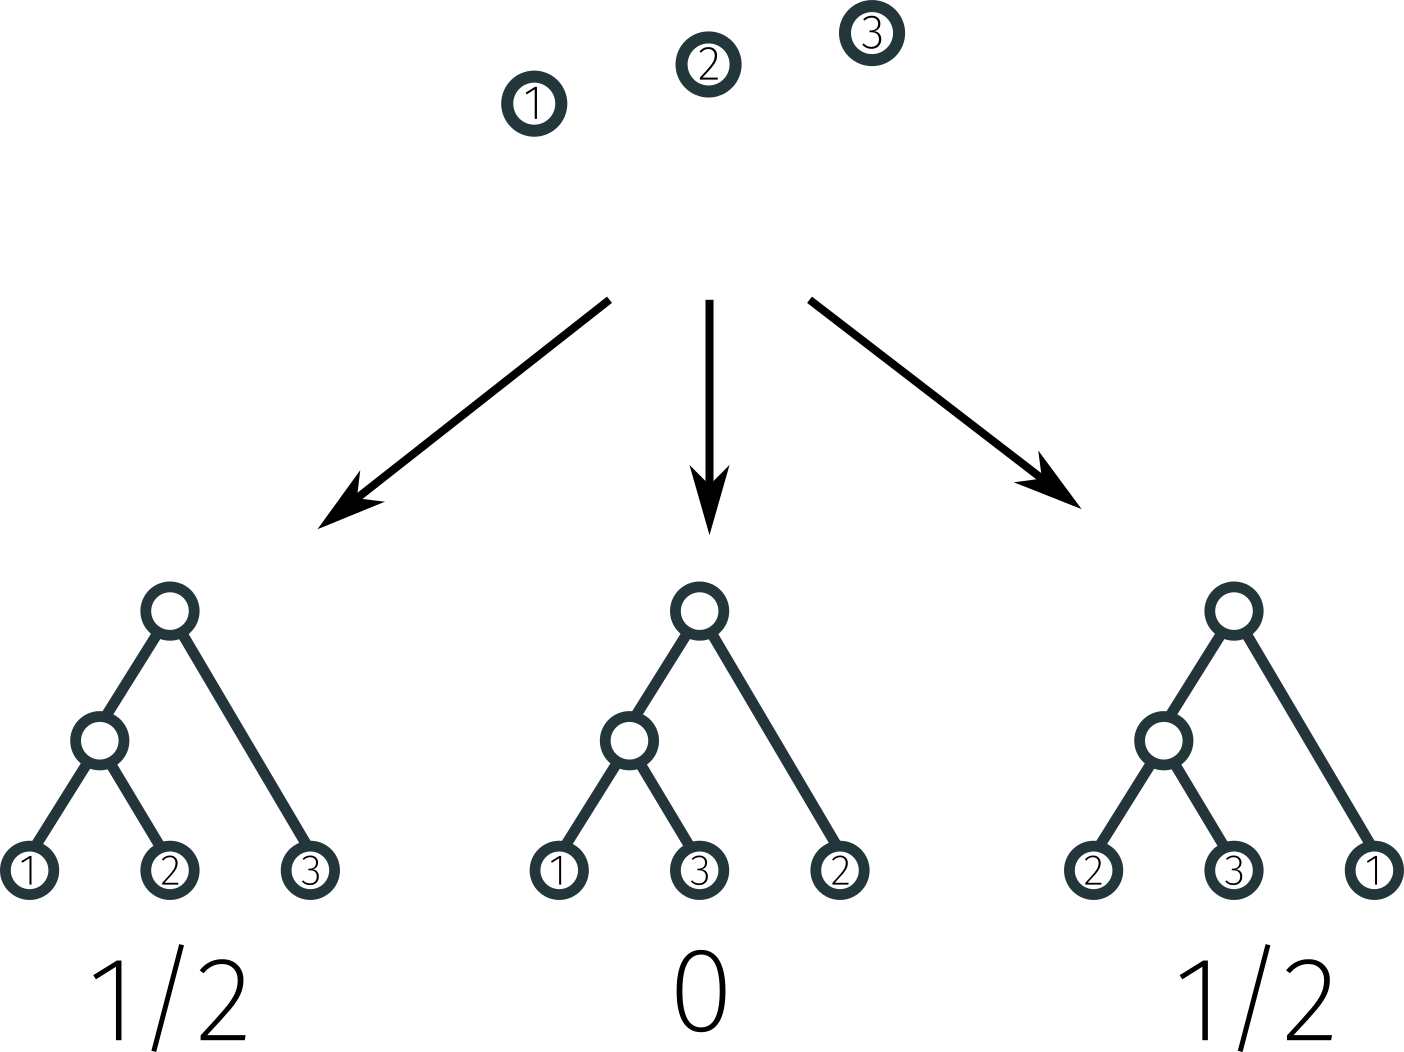
\includegraphics[width=0.7\textwidth]{img/structure/3-cluster-linear-distribution}
        \caption{}
    \end{subfigure}
    \caption{Examples of how Bayesian structure learning could resolve ambiguity in latent structure. In (a), all three possible clusterings are given equal probability and in (b), the two most likely clusterings split the probability.}
    \label{fig:ambiguous-structure-probability}
\end{figure*}

Bayesian structure learning can be formalized
as a latent variable model,
where we assume a prior over structures $\p(\structure)$,
and a likelihood model $p(\dataset \given \structure)$.
The goal is then to perform Bayesian
inference to obtain the posterior distribution $p(\structure \given \dataset)$. The simple graphical model for this generative process is pictured in \autoref{fig:graphical-model-bsl}.

\begin{figure}[htp!]
    \centering
    \includegraphics[]{tikz/lvm}
    \caption{The graphical model for Bayesian structure learning}
    \label{fig:graphical-model-bsl}
\end{figure}

The design space of Bayesian structure learning
amounts to first deciding a structure class (hierarchical clusterings, flat clusterings, linear dynamical systems, etc.) and additionally choosing a
particular prior distribution over the structures.
Although computing the posterior distribution $\p(\structure \given \dataset)$ amounts to Bayesian inference,
more often than not, this posterior distribution is analytically intractable and we must resort to
approximate inference. Thus, in practice, we must
also decide on an approximate inference algorithm (variational inference, MCMC, etc.).

\subsection{Bayesian linear dynamical system}

A Bayesian linear dynamical system (BLDS)
is an LDS with the addition of a prior
over the transition matrix and noise covariance. 
Although there are many choices of prior,
in this thesis, we use the matrix-Normal-inverse-Wishart (MNIW) prior, which is conjugate, details of which
are located in \autoref{sec:stats-mniw}.

The choice of this prior results in a generative model
\begin{align*}
    \dynmat, \dyncovar &\sim MNIW(\Psi, \dynmat_0, V, \nu) \\
    \state_{\t + 1} | \state_t, \dynmat, \dyncovar &\sim \N(\dynmat \state_t, \dyncovar)
\end{align*}
which is also visualized in \autoref{fig:graphical-model-blds}.

\begin{figure}[htp!]
    \centering
    \includegraphics[]{tikz/blds}
    \caption{The graphical model for a Bayesian linear dynamical system}
    \label{fig:graphical-model-blds}
\end{figure}

Because the MNIW prior is conjugate
with a linear dynamical system likelihood,
the posterior distribution $\p(\dynmat, \dyncovar \given \sequencen)$ is also MNIW
and can be computed in closed form.


We dedicate the next chapter to
Bayesian nonparametric hierarchical clustering.
%\section{Bayesian nonparametric hierarchical clustering}

%The first step in Bayesian structure learning
%for hierarchical clustering is identifying
%a class of structures. Then only can we specify
%a prior distribution over
%the structure class.

%The most basic structure in hierarchical clustering is a rooted binary tree with the data points at its leaves. This is sometimes called a {\it cladogram}. Very often, however, the tree is adorned with additional information, for instance:
%\begin{enumerate}
%\item An ordering of the internal nodes, where the root is assigned the lowest number and each node has a higher number than its parent.

%This ordering uniquely specifies the induced $k$-clustering (for any $k$): just remove the $k-1$ lowest-numbered nodes and take the clusters to be the leaf-sets of the $k$ resulting subtrees.

%\item Lengths on the edges.

  %Intuitively, these lengths correspond to the amount of change (for instance, time elapsed) along the corresponding edges. They induce a {\it tree metric} on the nodes, and often, the leaves are required to be at the same distance from the root. Cladograms with edge-lengths are referred to as \emph{phylogenies}.

%\item Parameters at internal nodes.

%These parameters are sometimes from the same space as the data, representing intermediate values on the way from the root to the leaves.
%\end{enumerate}
%Prior distributions over cladograms and phylogenies are a well-studied and
%developed area of Bayesian nonparametrics, and 
%We now review some well-known distributions over trees and over hierarchical clusterings.

%%Distributions over cladograms and phylogenies often take the shape of B
%%In this thesis, we focus on \emph{phylogenies}, which are rooted binary trees with data as leaves and edge-lengths.
%%Now that our structure class is decided, we must specify a prior distribution over phylogenies, for which we refer to
%%Bayesian nonparametrics, a branch of statistics concerned with distributions whose
%%complexity grows with the amount of data. These priors often take
%%the form of a generative process that builds a tree recursively and stochastically.

%Let's start with cladograms on $\numdata$ leaves. The simplest distribution over these is the uniform. Another well-studied option is the {\it Yule model}, which can be described using either a top-down or bottom-up generative process. The top-down view corresponds to a continuous-time pure birth process: start with one lineage; each lineage persists for a random exponential(1) amount of time and then splits into two lineages; this goes on until there are $\numdata$ lineages. The bottom-up view is a coalescing process: start with $\numdata$ points; pick a random pair of them to merge; then repeat. \citet{Aldous1995} has defined a one-parameter family of distributions over cladograms, called the {\it beta-splitting model}, that includes the uniform and the Yule model as special cases. It is a top-down generative process in which, roughly, each split is made by sampling from a Beta distribution to decide how many points go on each side. To move to arbitrary (not necessarily binary) splits, a suitable generalization is the Gibbs fragmentation tree~\citep{McCullagh2008}.

%In this thesis, we will work with joint distributions over both tree structure and data. These are typically inspired by, or based directly upon, the simpler tree-only distributions described above. Our primary focus is the Dirichlet diffusion tree~\citep{Neal2003}, which is specified by a birth process that we will shortly describe. However, our methodology applies quite generally. Other notable Bayesian approaches to hierarchical clustering include: \citet{Williams2000}, in which each node of the tree is annotated with a vector that is sampled from a Gaussian centered at its parent's vector; \citet{Heller2005}, that defines a distribution over flat clusterings and then specifies an agglomerative scheme for finding a good partition with respect to this distribution; \citet{Adams2008}, in which data points are allowed to reside at internal nodes of the tree; \citet{Teh2008, Boyles2012}, in which the distribution over trees is specified by a bottom-up coalescing process; and \citet{Knowles2011}, which generalizes the Dirichlet diffusion trees to allow non-binary splits. 

%\subsection{Dirichlet diffusion tree}

%The Dirichlet diffusion tree (DDT) is a 
%generative model for $d$-dimensional dataset
%$\dataset$. Data
%are generated sequentially via a continuous-time
%process, lasting from time $t = 0$ to $t = 1$,
%whereupon they reach their final value.

%The first point, $\x_1$, is generated
%via a Brownian motion, beginning at the origin, i.e.
%$X_1(t + dt) = X_1(t) + \N(0, \sigma^2I_ddt)$
%where $X_1(t)$ represents the value of $\x_1$ at time $t$.
%The next point, $\x_2$, follows the path created
%by $\x_1$ until
%it eventually \emph{diverges}
%at a random time, according to a specified
%acquisition function $a(t)$.
%When $\x_2$ diverges, it creates
%an internal node in the tree structure
%which contains both the time and value of $\x_2$
%when it diverged.
%After divergence, it continues until $t = 1$ with 
%an independent Brownian motion.
%In general, the $i$-th point
%follows the path created by the 
%previous $i - 1$ points.
%When it reaches a node, it
%will first sample one of two branches
%to enter, then
%either 1) diverge on the branch,
%whereupon a divergence time is sampled
%according to the acquisition function $a(t)$,
%or 2) recursively continue to the next node.
%Each of these choices has a probability
%associated with it, according to various properties
%of the tree structure and choice of acquisition function
%(details can be found in \citet{Neal2003}).
%Eventually, all points will diverge and continue independently,
%creating an internal node storing the time and
%intermediate value for each point at divergence.
%The DDT thus defines a binary tree over the data
%(see \autoref{fig:ddt} for an example).
%Furthermore, given a DDT with $N$ points,
%it is possible to sample the possible divergence
%locations of a $(N + 1)$-th point, using
%the generative process. 

%\begin{figure}[h]
    %\centering
    %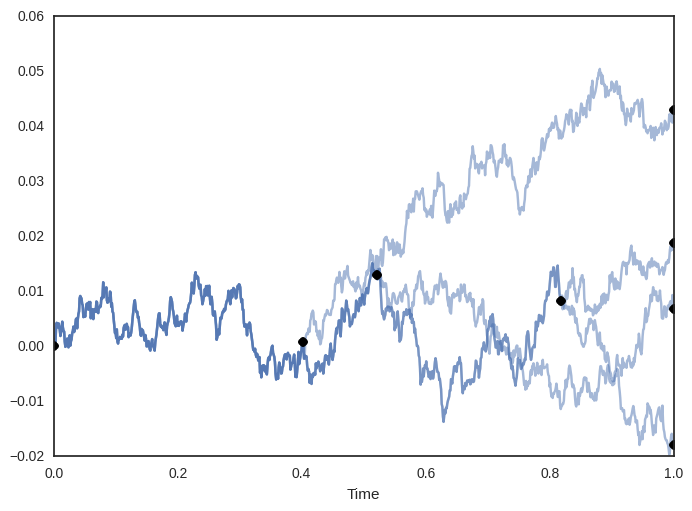
\includegraphics[width=0.45\textwidth]{img/ibhc/ddt}
    %\caption{An example DDT with 1-dimensional data. Blue lines represent paths
    %taken by each data point, and black dots represent nodes of the tree.
    %The rightmost dots are leaves and the others are nodes
    %created when points diverged. When drawing the hierarchy,
    %typically the top stem is omitted.}
    %\label{fig:ddt}
%\end{figure}


%This is accomplished via a simple recursive procedure.
%Let $u$ be the root of a subtree. 
%Let $v$ and $w$
%be the children of $u$, $\tt{leaves}(\cdot)$ 
%be the number of leaves descendant of a node,
%and $\tt{time}(\cdot)$ be the time associated with a node.
%\begin{itemize}
%\item Begin particle at $u$.
%\item Sample $v$ or $w$ proportional to $[\texttt{leaves}(v), \texttt{leaves}(w)]$. Let this
%sampled node be $s$.
%\item Sample whether or not divergence occurs according to $P(\text{diverge}) = 1 - \int_{\texttt{time}(u)}^{\texttt{time}(s)} a(t)/ \texttt{leaves}(s) dt$.
%\item If particle diverges, sample time between $\texttt{time}(u)$ and $\texttt{time}(s)$
%according to $a(t)$ and return $s$.
%\item If no divergence, recurse on $s$.
%\end{itemize}
%We choose $a(t)$ such that $a(1) = \infty$ so that
%divergence is guaranteed before recursing on a leaf.

%\subsection{Time marginalized coalescent}

%\subsection{MCMC inference}
%Sampling the posterior
%DDT given data can be done with the
%Metropolis-Hastings (MH) algorithm,
%an MCMC method.
%The MH algorithm 
%obtains samples from target distribution $p(\x)$
%indirectly by instead sampling
%from a conditional ``proposal'' distribution $q(\x | \x')$,
%creating a Markov chain whose stationary
%distribution is $\p(\x)$, assuming $q$ satisfies some conditions.
%Our choice of proposal distribution
%modifies the DDT's tree structure
%via a \emph{subtree-prune and regraft} (SPR) move,
%which has the added benefit of extending to
%other distributions over hierarchies.


%\subsubsection*{The Subtree-Prune and Regraft Move}
%\label{app:sprsampler}
%An SPR move consists of first a \emph{prune} then a \emph{regraft}.
%Suppose $\tree$ is a binary tree with $n$ leaves.
%Let $s$ be a non-root node in $\tree$ 
%selected uniformly at random and
%$S$ be its corresponding subtree.
%To prune $S$ from $\tree$, we 
%remove $s$'s parent $p$
%from $T$, and replace $p$ with $s$'s sibling.

%Regrafting selects a branch at random
%and attaches $S$ to it as follows. 
%Let $(u, v)$ be the chosen branch ($u$ is the parent of $v$).
%$S$ is attached to the branch by creating a node
%$p$ with children $s$ and $v$ and parent $u$ 
%(see \autoref{fig:sprmove} for an example).

%\begin{figure*}[htp!]
    %\centering
    %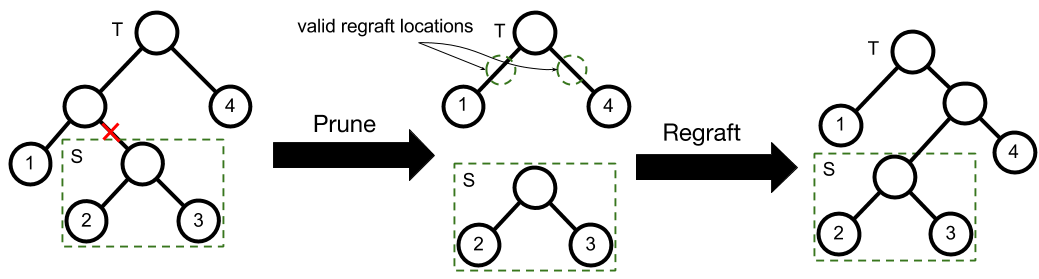
\includegraphics[width=\textwidth]{img/ibhc/SPRMove}
    %\caption{In the subtree-prune and regraft (SPR) move, a subtree $S$
        %is selected uniformly at random and is then pruned from the tree. 
            %Next, a regraft location is selected from the valid regraft locations, and $S$ is re-attached
            %at that location.}
    %\label{fig:sprmove}
%\end{figure*}

%The MH proposal distribution for the DDT
%is an augmented SPR move, where
%the time and intermediate value at each
%node are sampled in addition to tree structure.
%The exchangeability of the DDT enables
%efficient sampling of regraft branches by 
%simulating the generation process for a new point
%and returning the branch and time where it diverges.
%The intermediate values for the entire
%tree are sampled via an interleaved Gibbs sampling move,
%as all conditional distributions are Gaussian.
